\documentclass{article}

\usepackage{amsmath,amssymb}
\usepackage{tikz}
\usepackage{pgfplots}
\usepackage{xcolor}
\usepackage[left=2.1cm,right=3.1cm,bottom=3cm,footskip=0.75cm,headsep=0.5cm]{geometry}
\usepackage{enumerate}
\usepackage{enumitem}
\usepackage{marvosym}
\usepackage{tabularx}
\usepackage{multirow}
\usepackage[colorlinks = true, linkcolor = blue, urlcolor  = blue, citecolor = blue, anchorcolor = blue]{hyperref}

\usepackage{listings}
\definecolor{lightlightgray}{rgb}{0.95,0.95,0.95}
\definecolor{lila}{rgb}{0.8,0,0.8}
\definecolor{mygray}{rgb}{0.5,0.5,0.5}
\definecolor{mygreen}{rgb}{0,0.8,0.26}
\lstdefinestyle{java} {language=java}
\lstset{language=java,
	basicstyle=\ttfamily,
	keywordstyle=\color{lila},
	commentstyle=\color{lightgray},
	stringstyle=\color{mygreen}\ttfamily,
	backgroundcolor=\color{white},
	showstringspaces=false,
	numbers=left,
	numbersep=10pt,
	numberstyle=\color{mygray}\ttfamily,
	identifierstyle=\color{blue},
	xleftmargin=.1\textwidth, 
	%xrightmargin=.1\textwidth,
	escapechar=§,
}

\usepackage[utf8]{inputenc}

\renewcommand*{\arraystretch}{1.4}

\newcolumntype{L}[1]{>{\raggedright\arraybackslash}p{#1}}
\newcolumntype{R}[1]{>{\raggedleft\arraybackslash}p{#1}}
\newcolumntype{C}[1]{>{\centering\let\newline\\\arraybackslash\hspace{0pt}}m{#1}}

\newcommand{\E}{\mathbb{E}}
\DeclareMathOperator{\rk}{rk}
\DeclareMathOperator{\Var}{Var}
\DeclareMathOperator{\Cov}{Cov}
\DeclareMathOperator{\SD}{SD}
\DeclareMathOperator{\Cor}{Cor}

\title{\textbf{Instrumente des Finanzmanagements, Tutorium 4}}
\author{\textsc{Henry Haustein}}
\date{}

\begin{document}
	\maketitle
	
	\section*{Aufgabe 18: Arbitrage-Pricing-Theorie}
	\begin{enumerate}[label=(\alph*)]
		\item Long Wertpapier 2 mit Gewicht 2, Short Wertpapier 1 mit Gewicht -1. Damit sind die Betas
		\begin{align}
			\beta_{1,P} &= 2\cdot 0.5 - 1 = 0 \notag \\
			\beta_{2,P} &= 2\cdot 2 - 1.5 = 0.5 \notag
		\end{align}
		Damit ist die erwartete Rendite ist
		\begin{align}
			\E(r_P) &= 2\left(20\% + 0.5\cdot\underbrace{\E(F_1)}_{0} + 2\cdot\underbrace{\E(F_2)}_{0}\right) - 1\left(20\% + 1\cdot\underbrace{\E(F_1)}_{0} + 1.5\cdot\underbrace{\E(F_2)}_{0}\right) \notag \\
			&= 40\% - 20\% \notag \\
			&= 20\%\notag
		\end{align}
		\item Long Wertpapier 3 mit Gewicht 3, Short Wertpapier 4 mit Gewicht -2. Damit sind die Betas
		\begin{align}
			\beta_{1,P} &= 3\cdot 1 - 2\cdot 1.5 = 0 \notag \\
			\beta_{2,P} &= 3\cdot 0.5 - 2\cdot 0.75 = 0 \notag
		\end{align}
		Damit ist die erwartete Rendite ist
		\begin{align}
			\E(r_P) &= 3\left(10\% + 1\cdot\underbrace{\E(F_1)}_{0} + 0.5\cdot\underbrace{\E(F_2)}_{0}\right) - 2\left(10\% + 1.5\cdot\underbrace{\E(F_1)}_{0} + 0.75\cdot\underbrace{\E(F_2)}_{0}\right) \notag \\
			&= 30\% - 20\% \notag \\
			&= 10\%\notag
		\end{align}
		\item Auch das Portfolio in (b) ist unabhängig von $F_1$ und $F_2$. Man leiht sich also Geld mit 5\% Zinsen und kauft damit das Portfolio (b).
		\item Der Zins $r_f$ wird steigen und die Rendite von dem Portfolio in (b) wird sinken, bis keine Arbitragemöglichkeit mehr vorhanden ist.
	\end{enumerate}

	\section*{Aufgabe 13.2: Wettbewerb und Kapitalmärkte}
	\begin{enumerate}[label=(\alph*)]
		\item Durch einen höheren risikofreien Zinssatz verändert sich das Marktportfolio. Damit ist das alte Marktportfolio nicht mehr effizient.
		\begin{center}
			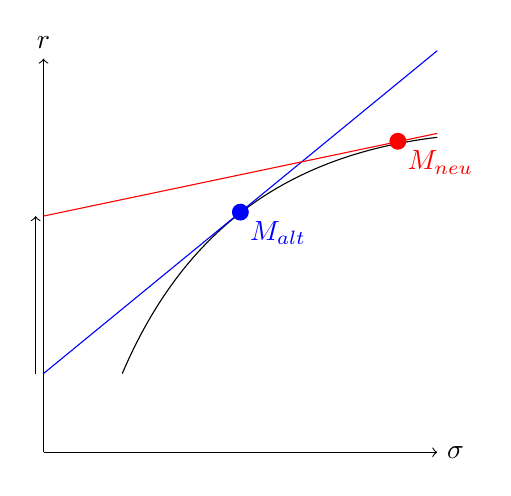
\begin{tikzpicture}
				\draw[->] (0,0) to (5,0) node[right] {$\sigma$};
				\draw[->] (0,0) to (0,5) node[above] {$r$};
				
				\draw (1,1) to[bend left=30] (5,4);
				\draw[blue] (0,1) -- (5,5.1);
				\draw[blue,fill=blue] (2.5,3.05) circle (0.1) node[below right] {$M_{alt}$};
				\draw[red] (0,3) -- (5,4.05);
				\draw[red,fill=red] (4.5,3.95) circle (0.1) node[below right] {$M_{neu}$};
				\draw[->] (-0.1,1) -- (-0.1,3);
			\end{tikzpicture}
		\end{center}
		\item Im Marktportfolio sind nun Aktien mit mehr Risiko und Rendite, das heißt solche Aktien werden gekauft, während Aktien mit wenig Rendite und Risiko verkauft werden.
	\end{enumerate}

	\section*{Aufgabe 13.3: Informationen und rationale Erwartungen}
	Marktportfolio kaufen

	\section*{Aufgabe 13.11: Systemische Verzerrungseffekte beim Handeln von Wertpapieren}
	\begin{enumerate}[label=(\alph*)]
		\item alle verkaufen ihre Aktien bei einem Preis von 55\EUR\,$\Rightarrow$ das ist der Gleichgewichtspreis
		\item Wenn der Preis der Aktie auf 55\EUR\, steigt, dann ist eine Übernahme wahrscheinlich und wir kaufen die Aktien, weil die Aktie bald 60\EUR\, wert ist.
	\end{enumerate}

	\section*{Aufgabe 13.16: Markt-Anomalien und die Debatte über die Markteffizienz}
	\begin{enumerate}[label=(\alph*)]
		\item Der Marktwert ist $\frac{Div}{r}$, damit sind die Unternehmenswerte:
		\begin{align}
			BW_{S1} &= \frac{10\text{ Mio. \EUR}}{0.08} = 125\text{ Mio. \EUR} \notag \\
			BW_{S2} &= \frac{10\text{ Mio. \EUR}}{0.12} = 83.3333\text{ Mio. \EUR} \notag \\
			BW_{S3} &= \frac{10\text{ Mio. \EUR}}{0.14} = 71.4286\text{ Mio. \EUR} \notag \\
			BW_{B1} &= \frac{100\text{ Mio. \EUR}}{0.08} = 1250\text{ Mio. \EUR} \notag \\
			BW_{B2} &= \frac{100\text{ Mio. \EUR}}{0.12} = 833.3333\text{ Mio. \EUR} \notag \\
			BW_{B3} &= \frac{100\text{ Mio. \EUR}}{0.14} = 714.2857\text{ Mio. \EUR} \notag
		\end{align}
		\item Long S1 mit einem Gewicht von 1, Short S3 mit einem Gewicht von -1 $\Rightarrow r=8\% - 14\%=-6\%$ \\
		Long B1 mit einem Gewicht von 1, Short B3 mit einem Gewicht von -1 $\Rightarrow r=8\% - 14\%=-6\%$
		\item Long B1 mit einem Gewicht von 1, Short S3 mit einem Gewicht von -1 $\Rightarrow r=8\% - 14\%=-6\%$
		\item Long B3 mit einem Gewicht von 1, Short S1 mit einem Gewicht von -1 $\Rightarrow r=14\% - 8\%=6\%$
	\end{enumerate}
	
\end{document}